\chapter{Problem Analysis}
\label{chapter:concept}
This chapter analyzes the current state of the application and identifies problems that occur when using AMCS via a web browser on mobile
devices. To narrow down the extend of this work, the system is analyzed from the point of view that an audience member like a student has while using AMCS on their smartphone. While doing so, students will interact mostly with the \emph{Main View}, the \emph{Poll View} and the \emph{Navigation / Burger Menu}. Therefore, this work is centered around but not limited to these components (see \Cref{tab:components}).

\section{Problems Of The Mobile View}
\label{section:con:problems}
The back end of AMCS reacts on requests coming from mobile devices such as smartphones or tablets by providing a responsive mobile view to its clients. However, in some aspects, AMCS struggles to offer a uniform UI experience that guarantees the best usability possible.
One challenge lies in the fact that the system has to deal with limited screen space to visualize information with maximum effectiveness. Decisions have to be made on the size and placement of different UI components depending on the information that they should convey to the user.
\\
\\
User interaction likewise plays a big role. Some users might approach the application with different ways of interaction and navigation that are characteristic for mobile devices. For example, a smartphone user might expect to be able to use swiping gestures to navigate a menu. The user could also expect that information is organized in views consisting of separate tabs, which is a typical technique used to display a lot of information on limited screen estate.
\\
\\ 
This section lists key issues that lower usability or might cause confusion to mobile users in the sense described above. A tabular summary of the findings can be found in \Cref{tab:problems2}.

\subsection{Main View}
As already described in \Cref{section:soa:mainview}, the \emph{Main View} relies on a vertically scrolling list view, consisting of different sections. While this is the most intuitive design to chose for use on smartphones, details of the implementation in place cause problems and impair the usability of the application.

\subsubsection{General Visualization Problems}
\label{section:con:problems:mainview:generalvis} \Cref{section:soa:mainview:lectures} covered the fact, that lectures are rendered by displaying the title of the lecture in the top section of the box using white letters on a solid blue background. It is followed by details about the lecture such as time, duration and a textual description, visualized in gray letters and icons on a white background. Finally, at the bottom of the box, the course name is shown in gray letters on a light blue background. The order \emph{lecture name, details, course name} can cause confusion.
The most coarse grain piece of information - the course name - is displayed at the bottom of the box rather than at the top. Generally, when seeking information about active lectures, a student will most likely remember the course name rather than the name of a single lecture, as timetables used by students only contain course names. Therefore, displaying the information in this order could lead to students take longer time to find the pieces of information that they are looking for.

In addition to that, inappropriate background colors and font sizes are used to differentiate between course name and lecture name, further increasing the ambiguity described above.

To sum it up, the hierarchical and logical relationship between courses and lectures is disregarded in the way this information is visualized. 

\subsubsection{No Notifications For New Or Unread Content}
\label{section:con:problems:noindicators}
A commonly used technique to lead the user to new content is an \emph{Unread Content Indicator} (see \todogrf{facebook indicator}).
The \emph{Main View} lacks completely of indicators of any kind for new or unread content. This is a problem because typically, not all polls are visible to students at the beginning of a semester - either because the polls do not exist yet or for the reason that polls can be activated by lecturers at a preferred point in time. For example, in order to see whether or not for a given course or lecture new polls exist, students have to tap on the lecture to check. This is unintuitive and adds another layer of indirection to the overall workflow.

\subsubsection{Indirection Problems}

The boxes that represent each lecture claim a lot of screen space in relation to the information that is displayed to the student (see \Cref{fig:mainview}). The layout causes plenty of indirection, because per default, the sections for upcoming and active lectures are expanded fully. This might be handy when quickly gathering information about lectures that are or soon will be active, but in every other case it slows navigation and overall interaction, because the \emph{Course Management} section is pushed down to the bottom.
A list of only four boxes causes a scroll bar to appear on the very common screen resolution of 1920x1080 pixels. A student that navigates to the \emph{Main View} to enroll into a new course therefore has to scroll to the bottom of the page before they reach the \emph{Enrollment Form}. The same problem occurs when simply seeking information about what courses a student is already enrolled in or when trying to leave a course altogether. 
\\
\\
Furthermore, if a student seeks information regarding a specific course, no filter or search functionality is offered by the lecture list. Instead of typing the course name in a search bar, they have to scroll down to the bottom of the lecture list, scan the course list manually with their eyeballs, find the course and click on the corresponding item. After that, they are redirected to the \emph{Course View}, which then displays a filtered list of lectures belonging to the course. The level of indirection is further increased the more courses the student is enrolled in. 

\subsubsection{Redundancy}

Some visual redundancy is added by the badges that are displayed on the upper-right corner of each lecture. These badges are used to visualize the temporal context of the lecture for each item in the corresponding section. It seems that the badge's were introduced as an additional means to help conveying the temporal context of the lecture, because sorting the lectures in their respective section alone fails to do so.
Yet the badge's names do not match the section's names, e.g. an upcoming lecture's badge reads \emph{BEFORE} instead of \emph{UPCOMING}. 

Some visual redundancy can also be found in the \emph{Course Management} section below. Each course is represented by a box with the course's name along with an unsubscribe button, represented by a trash can icon (see\Cref{fig:mainviewcoursemanagement}). This is a redundant way of rendering the courses, as repetition (especially of the trash can icon) adds noise to the overall look. Plenty of the vertical screen estate is wasted in this manner.
\subsection{Course View}
\label{section:con:problems:courseview}
Since the \emph{Course View} reuses the lecture list along with the sections \emph{Upcoming lectures}, \emph{Active lectures} and \emph{Past lectures}, likewise the same issues arise as for the \emph{Main View}, as already described in \Cref{section:con:problems:mainview:generalvis}. 
The \emph{Course View} has a very important function in terms of usability due to it acting as a filter for lectures that belong to a certain course. Problems arise when a user wants to switch quickly between different courses. Doing so requires to leave the \emph{Course View} by tapping the back button and then scanning the \emph{Course Management} section for the element of interest, which is slow and cumbersome. This is explained in more detail in \Cref{section:con:problems:navigation}

\subsection{Poll View}

\subsubsection{Visualization}
\label{section:con:problems:pollview}

\Cref{section:soa:pollview} describes the rendering of questions as boxes that are aligned in a vertical scrolling list. Namely the extensive use of vertical space on the screen is one problem introduced by this layout. Bigger polls that consist of multiple questions unnecessarily take plenty of vertical screen estate. 
Answering one question usually does not require to see the neighboring questions, but most of the time, two to three questions are in view simultaneously (see \Cref{figure:pollview}). This might be distracting to some students.

The view also lacks of basic but potentially interesting information such as the number of total and remaining questions. This information might be useful in bigger polls if students want to gain an idea on how many questions are left.

In general, the layout lacks of separation and distinction between individual types of polls.
Polls of the same type are separated by a heading that denotes the poll type. Each group of polls is then simply appended to the bottom of the list, increasing its length even further.
\todogrf
\subsubsection{Local Navigation}

The vertical list is difficult to navigate as it requires scrolling between questions. If a student wants to jump from the first to the last question, or vice versa, several swiping gestures are needed to reach the top or the bottom of the list.
Similar to the lecture list described in \Cref{section:soa:mainview:lectures}, the question list is also segmented into different sections. Lecture and course questions are similarly appended to the bottom of a \emph{Slide Poll}. This layout requires that a student who wants to view these questions has to scroll all the way to the bottom of the list, further increasing indirection and slowing interaction down.



\subsection{Burger Menu and Navigation}
\label{section:con:problems:navigation}

At the time of writing, the ways of navigating the application can be described as problematic and partly confusing. Several layers of indirection introduce problems and may worsen the user experience.
\Cref{figure:clickpathproblems} illustrates click paths a user must take in order to reach different views (illustrated in blue) within AMCS. In general, some views are connected via the \emph{Burger Menu} as the overarching element of navigation (illustrated in green). In contrast, other views are interconnected and can be reached by clicking on elements inside a view such as a course or lecture. The following paragraphs elaborate more on both aspects of navigation.
\newline
\newline
On the one hand, the interconnected graph of views as it is described in \Cref{figure:clickpathproblems} contains two bigger issues. One example of unexpected behavior is the path that a user takes when he wants to return from the \emph{Poll View} to the \emph{Main View} in order to choose a different poll.
It is possible to reach the \emph{Poll View} from the \emph{Main View} with only one tap, for example by selecting a lecture.
However, by pressing the back button, the user is first redirected to the \emph{Course View} and then, with a second tap on the back button, to the \emph{Main View}. A more well defined implementation would rather directly return to the last element of the \emph{View Stack}, in this case the \emph{Main View}.
 
Furthermore, some views like the \emph{Question Pool View} and the \emph{Answer Evaluation View} do not offer buttons that allow to navigate back. The navigation therefore relies partly on the corporate branding on the upper-left that when tapped will redirect to the \emph{Main View}.
This means that the interconnectedness between different views might not be strong enough.
\newline
\newline
On the other hand, the \emph{Burger Menu} that connects several aspects and functionalities of AMCS in an overarching manner (as it is part of every view) has it's own issues. 
One visual problem that arises is the fact that the menu excessively uses vertical screen space and delocates the rest of the content that is currently shown when several sub menus are expanded. A reason for why this is problematic might be the following scenario: a student wants to evaluate their answers to polls for a certain lecture. When opening the menus on their phone from the \emph{Main View}, information like course name and lecture title are pushed down by the menu, potentially completely out of the viewport. But this information is required in the \emph{Answer Evaluation View} because the user is asked to choose their course and lecture of interest from two drop down menus. This could lead to users having to return to the \emph{Main View} to look up the lecture name or other details again so that they can proceed with their selection.
\\
\\
An additional, different issue arises from the labeling of menu entries. The labels can confuse students because the first menu entry is labeled as \emph{Student}. This implies in general that different user roles exist in AMCS, which is the case. However the user's role should not be the label of a sub menu in the navigation. While functionality like \emph{Account management} might be a plausible function to be found here, it is rather unintuitive that the \emph{Question Pool} and \emph{Answer Evaluation} can be accessed via a button labeled \emph{Student}.

\subsubsection{Evaluation of answers}

As mentioned above, tapping on the option \emph{Evaluation of answers} in the expanded \emph{Burger Menu} leads to a view with a drop down menu from which students can choose a course that they are interested in. Afterwards, a list of expandable items is shown, where each item represents a lecture. Clicking on one or multiple of these items will expand a vertical list of questions similar to the regular question list described in \Cref{section:con:problems}. Likewise, answers given by the student are shown as well (see Fig. \todogrf).
Multiple problems occur on this view: First of all, the navigation path to reach this view contains unnecessary indirection and might not be intuitive enough, which is illustrated by \Cref{figure:clickpathproblems}. Students might expect this functionality to be located at the \emph{Main View} attached to the elements of the course list or inside the \emph{Course View} itself. Instead, every time evaluation of given answers is attempted, this functionality can only be accessed by using the \emph{Burger Menu}, choosing the appropriate item from the sub menu, selecting the course in question and afterwards expand the lecture and the corresponding question list.
Moreover, the question list suffers from the same rendering and navigation problems already described in \Cref{section:con:problems:pollview}. Questions are poorly navigable and a good of scrolling is required to jump between questions.


\begin{figure}[ht]
	\centering
	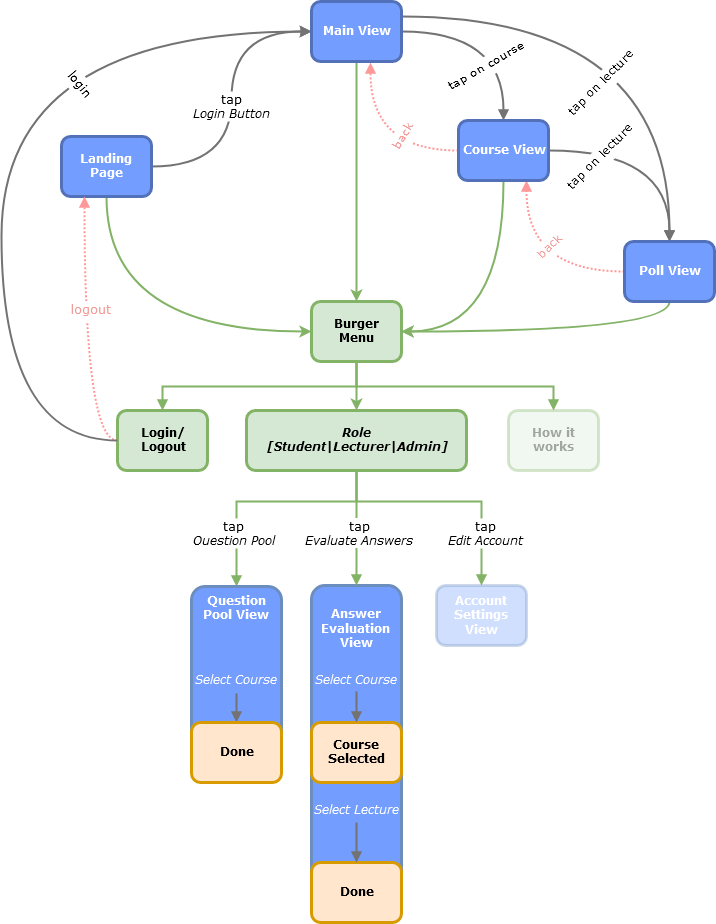
\includegraphics[width=\textwidth]{diagrams/amcs-click-paths.png}
	\caption{Navigation concept of AMCS: Every arrow represents a tap / click the user has to do to reach the desired destination.}
	\label{figure:clickpathproblems}
\end{figure}

\begin{figure}[ht]
	\centering
	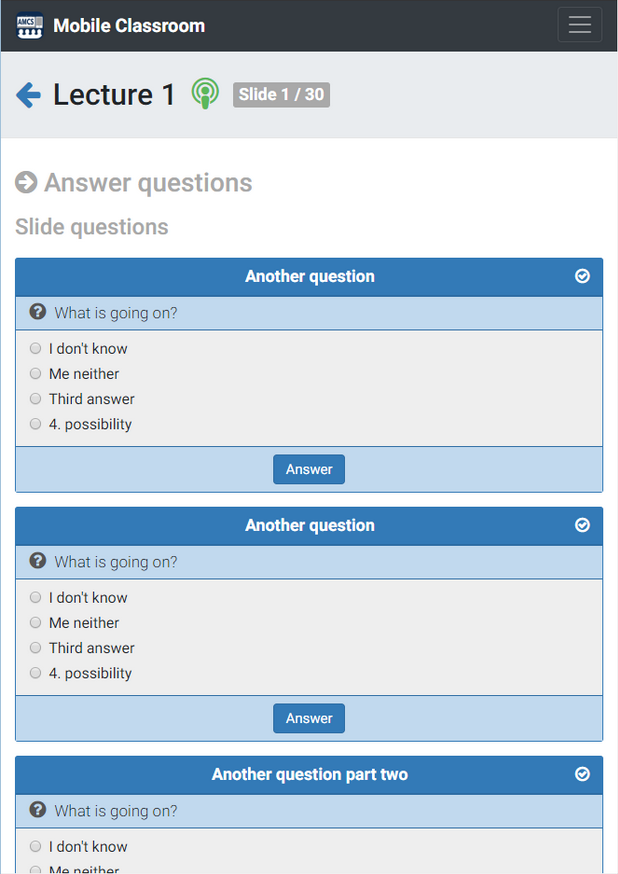
\includegraphics[width=0.5\textwidth]{screenshots/poll_view_2.png}
	\caption{\emph{Poll View}: Multiple questions are displayed at the same time.}
	\label{figure:pollview}
\end{figure}
\subsubsection{Question Pool}

The question pool suffers from the same navigation problems described in the preceding section. Again, a drop down menu for selecting a course is shown before students can see the overview of the \emph{Question Pool}. Once more, students might think that access to this functionality is located near the \emph{Main View} or the \emph{Course View}, which is not the case.
\cleardoublepage
\renewcommand*{\arraystretch}{1.4}
\begin{longtable}{ | p{1.1cm} | p{2cm} | p{2cm} | p{2.5cm} | p{5.5cm} |}
\hline
ID & Name & Categories & Components & Summary \\ \hline \hline
GV 1 & Visualization of Lectures & Visualization & Main View & The hierarchical order of courses containing lectures is disregarded. \\ \hline
GV 2 & Missing Notifications & Visualization & Main View, \newline Course View & No notifications for new or unread content are given. \\ \hline
GV 3 & Lecture Badges & Visualization, \newline Redundancy & Main View, \newline Course View & Lecture badges that indicate temporal context are redundant and do not match their respective section in the lecture list. \\ \hline
GV 4 & Course List & Visualization, \ Redundancy & Main View & Courses are each rendered in a box as a list on the bottom of the \emph{Main View}. \\ \hline
IN 1 & Course Management & Layout & Main View & The section \emph{Enrollment} and the course list are located too far to the bottom of the view. \\ \hline
IN 2 & Course Filter & Functional & Main View & The view lacks of a filtering mechanism. \\ \hline
PV 1 & Poll View Layout & Visualization \newline Layout & \emph{Poll View} & The poll layout uses too much vertical space. \\ \hline
PV 2 & Missing Poll Information & Visualization & \emph{Poll View} & The number of total and remaining questions is missing. \\ \hline
PV 3 & Missing Poll Separation & Layout, \newline Navigation & \emph{Poll View} & The view lacks of separation between different poll types. Navigation between different poll types requires too much scrolling. \\ \hline
NAV 1 & Switching Courses & Navigation & Main View, \newline Course View & Quickly switching between courses requires unnecessary navigation between \emph{Course View} and \emph{Main View}. \\ \hline	
NAV 2 & Confusing Click Paths & Navigation & \emph{Main View, \newline Course View, \newline Poll View} & Under certain circumstances, returning to an earlier view can yield unexpected results. \\ \hline
NAV 3 & Weak View Interconnectedness & Navigation & \emph{Main View, \newline Question Pool View, \newline Answer Evaluation View} & Some views miss proper back buttons to return to the previous view. \\ \hline
NAV 4 & Menu Size & Visualization \newline Layout & \emph{Burger Menu} & Fully expanding the \emph{Burger Menu} uses too much screen space. \\ \hline
NAV 5 & Menu Labeling & Visualization & \emph{Burger Menu} & Some menu entries are labeled inadequately. \\ \hline			
NAV 6 & Evaluation of Answers & Navigation \newline Layout & \emph{Answer Evaluation View} & Several drop down menus must be operated to evaluate answers for a given lecture. \\ \hline	
NAV 7 & Question Pool & Navigation & \emph{Question Pool View} & The \emph{Question Pool View} is not reachable easy enough, as expanding the \emph{Burger Menu} is required. \\ \hline									

\caption{Classification of issues identified in the usability analysis of AMCS.}
\label{tab:problems2}
\end{longtable}

